\chapter{Analyze Honeypot Attacks in the Cloud}
\label{chap:cloud-security}

Attacks from the Internet are often originated from bots.
A bot, short for \enquote{robot}, is an automated process that interacts with different network services.
Besides good intentions, bots can be used for malicious purposes.
Mostly, bots try to self-propagate malware across the Internet and try to capture hosts that merge into a botnet.
A botnet has a central server or servers that act as a command and control center for all infected hosts \cite{Feily2009}.
Recently, Universities in Germany received more cyberattacks than ever, respectively increasing their costs for damage repairs.
Honeypots are a good solution to catch attackers and learn from their exploits.
However, there is no conclusion if honeypots in times of bots give a proper countermeasure to avoid such damage.
Following the rise of cyberattacks, we introduce a method to collect and analyze cyberattacks in a cloud environment.
We further propose an answer if honeypots are helpful to prevent such scenarios from happening.

\section{Introduction}

As previously mention in \autoref{sec:cloud-computing}, using cloud resources are becoming the go-to option for new services and applications.
\citet{Kelly2021} thoroughly investigated honeypots on Azure, \ac{aws}, and \ac{gcp}.
Followingly, we present their results that we want to compare on with the ones heiCLOUD achieves.
The results are collected by T-Pot version $20.06.0$ over a duration of 3 weeks.
In addition, \citet{Kelly2021} considered different server geographical locations.
They have collected data from East US, West Europe, and Southeast Asia.
\autoref{tab:overview-cloud-security} shows the results presented by \citet{Kelly2021}.
Dionaea (a honeypot to capture malicious payload), Cowrie (SSH and Telnet honeypot), and Conpot (industrial honeypot for \acs{ics}, and \acs{scada}) are the most attacked honeypots in comparison to the others.
Regarding \ac{aws}, Dionaea account $91\%$ of the total attacks, Glutton and Cowrie are minor with $5\%$, and $2\%$.
Interestingly, Cowrie reported several attacks related to the COVID-19 pandemic to enable social engineering methods.
In contrast to \ac{aws}, Cowrie logged the majority of attacks with $51\%$ on \ac{gcp}.
Beside several automated attacks trying to log in with default credentials, adversaries tried to gather information about CPU architecture, scheduled tasks, and privilege escalation.
Microsoft Azure reflects nearly the same results as the other two cloud providers beforehand.

\begin{table}
    \centering
    \caption[Overview of attacks on cloud providers]{Overview of attacks on cloud providers. For a better overview, only the three most attacked honeypots are listed. The others combine several honeypots.}
    \begin{tabularx}{\linewidth}{l|XXXX|l}
        \toprule
        \textsc{Provider} & \multicolumn{4}{c|}{\textsc{Honeypot}} & \textsc{In Total}                                                   \\
                          & \textbf{Dionaea}                       & \textbf{Cowrie}   & \textbf{Glutton} & \textbf{others} &            \\
        \hline
        \acl{aws}         & $228\,075$                             & $4\,503$          & $11\,878$        & $3\,688$        & $248\,144$ \\
        \acl{gcp}         & $162\,570$                             & $297\,818$        & $84\,375$        & $36\,403$       & $581\,116$ \\
        Microsoft Azure   & $308\,102$                             & $9\,012$          & $17\,256$        & $6\,365$        & $340\,735$ \\
        \bottomrule
    \end{tabularx}
    \label{tab:overview-cloud-security}
\end{table}

The overall results show an average ratio of $55.000$ attacks per day, summing up to roughly $1.3$ million in total.
Similar results for different regions could have been reproduced.
Their results clearly show the disparity of the regions Europe, US, and Asia.
An important question that \citet{Kelly2021} answered is if attackers target services on cloud providers based on the cloud providers' market share.
They could not confirm this assumption based on the fact that Google Cloud with the smallest market share received most of the attacks.
In total, most of the attacks are originated from Vietnam, Russia, United States, and China.
Due to technologies such as VPN, or Tor, the geolocation only indicates the last node, so location data might be distorted.
Across all providers roughly $80\%$ of the source IP addresses had a bad reputation and could have been filtered by the organization.
The operating devices used for attacking the services are mostly Windows 7 or 8, and different Linux kernels and distributions.
Windows devices target vulnerabilities in remote desktop sharing software. Such vulnerabilities are
\begin{enumerate*}[label=(\roman*)]
    \item CVE-2006-2369\cite{CVE-2006-2369} (RealVNC) in the US region,
    \item CVE-2001-0540\cite{CVE-2001-0540} (RDP) in EU and Asia regions,
    \item CVE-2012-0152\cite{CVE-2012-0152} (RDP) in the Asia region, and
    \item CVE-2005-4050\cite{CVE-2005-4050} (VoIP) in EU region
\end{enumerate*}.
In addition, attackers were also capable of disguising any fingerprinting activity of p0f.

We want to compare the findings \citet{Kelly2021} claimed in the paper \enquote{A Comparative Analysis of Honeypots on Different Cloud Platforms} with ours using the University Heidelberg's cloud solution.
First, a short introduction of heiCLOUD is held, followed by a closer lookup of T-Pot that is used to acquire data.
Lastly, we present our results and do a thorough comparison closing up with a discussion based on a technical report of the Cambridge University.

\section{Methodology}

Our foremost goal is to track as most attacks as possible.
We want to verify if most of the attacks on the Internet are originated from bots.
To gather various attacks from the Internet \autoref{fig:concept} sketches our concept we plan to apply.
Honeypots should be deployed on a single instance, and store their data, or log files in a database.
By the help of data visualization tools, we analyze the attacks.
For security reasons, honeypots should run in a virtualized environment to avoid any harm to our host system.
We use Debian as a base Linux distribution.
Our instance runs on heiCLOUD, a cloud service provided by Heidelberg University.
It is capable of 16 GB of RAM, 8 VCPU's, and a volatile memory of 30 GB.
In addition, we mount a 125 GB permanent memory to securely store our data.
In its very early stages, we compared different approaches to achieve this goal.
As an example, we compared native implementation approaches, using additional frameworks, and ready-to-use solutions.
However, the T-Pot, developed by Telekom, offers a profoundly ready-to-use solution with major advantages.
It combines several honeypots in conjunction with various analytic tools to trace the newest attacks.
Furthermore, it helps to compare our findings with the ones \citet{Kelly2021} claim.

\begin{figure}[ht]
    \centering
    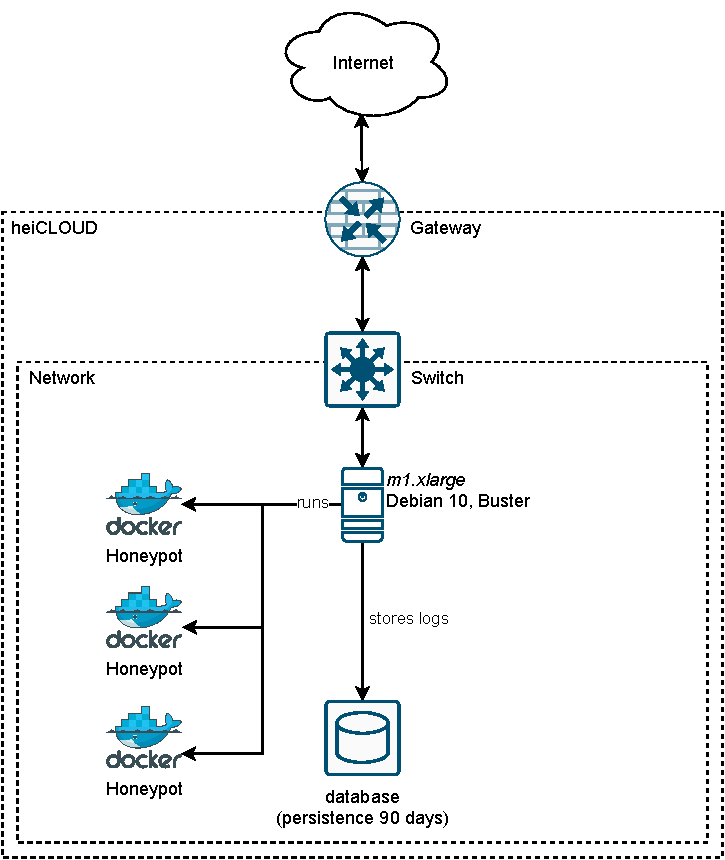
\includegraphics{figures/tpot-concept.pdf}
    \caption[Draft for data collection]{Concept to collect honeypot attacks}
    \label{fig:concept}
\end{figure}

Running our instance and exposing it to the Internet needs some adjustments beforehand.
Therefore, a virtual network with subnet \ipAddress{192.168.145.0/24} has been created wherein our instance with IP address \ipAddress{192.168.145.4} is assigned to.
The instance is accessible from the outside with floating IP address \ipAddress{129.206.5.74}.
Access rules are similar to a stateful firewall, and thus, do not block any attacks.
Ports $1-64000$ are exposed and can be attacked by anyone.
Ports higher than $64000$ are only accessible through the University network \ipAddress{129.206.0.0/16} or eduroam \ipAddress{147.142.0.0/16} and should provide a basic authentication with username and password.

\subsection{heiCLOUD}
\label{subsec:heicloud}

\citet{urz2021} offers a \enquote{\ac{iaas} specially tailored for higher education and research institutions} called heiCLOUD.
It supplies multiple institutes at Heidelberg University with storage, virtual machines, or network components.
In addition, heiCLOUD is a DFN\footnote{German National Research and Education Network, the communications network for Science and research in Germany} member, and offers others to use their services.
As stated on their information website\cite{heicloud2021}, it is
\begin{enumerate*}[label=(\roman*)]
    \item capable of freely manageable IT resources,
    \item beholds a stable and fast connection,
    \item ensures high availability and scalability,
    \item has freely selectable VM operating systems, and
    \item has a transparent payment model
\end{enumerate*} \cite{heicloud2021}.
Based on the open source application OpenStack, users can easily create own network areas, and manage their space individually.
Unlike well-known cloud providers, heiCLOUD servers are located withing Germany, thus, abide by the European data privacy law.
HeiCLOUD have never considered honeypots for additional cybersecurity measurements.

\subsection{T-Pot}
\label{subsec:tpot}

To be able to compare our results with \citet{Kelly2021}, we use the same approach to capture recent cyberattacks.
The T-Pot solution, a mixture of Telekom and Honeypot, stands out with their sheer quantity of various honeypots.
It requires $8$ GB RAM and a minimum of $128$ GB hard drive storage.
Based on a Debian 10 Buster distribution, it relies on Docker to run their services \cite{docker2021}.
T-Pot has to be deployed in a reachable network where intruders are expected.
Either TCP and UDP traffic are forwarded without filtering to the network interface, or it runs behind a firewall with forwarding rules.
Specified ports for attackers are $1$-$64000$, higher ports are reserved for trusted IPs, thus, a reverse proxy asks for basic authentication.
All daemons and tools run on the same network interface whereas some of them are encapsulated in their own Docker network.
Docker is a lightweight virtualization technology that uses containers to run on the host system \cite{combe2016}.
Unlike virtual machines, Docker reduces overhead with the downside of a greater attack surface.
To mitigate attacks, Docker wraps containers in an isolated environment.
This is achieved by restricting the kernel namespace and control groups (\verb|cgroups|).
\autoref{fig:overview-tpot} visualizes the technical concept of T-Pot.
Each service has dedicated ports or port ranges that are exposed.
Attackers can communicate either with TCP or UDP.
All honeypots and tools create log files that are used to get any knowledge about attackers.
In order to view and trace current attacks, T-Pot uses the ELK stack.
ELK is the acronym of Elasticsearch, Logstash and Kibana \cite{elastic2021}.
Elasticsearch is a search engine based on Lucene.
It is multitenant-capable and offers full-text search via HTTP.
Logstash is used to feed Elasticsearch.
In general, it offers an open server-side data processing pipeline that helps to send data from multiple sources to an Elasticsearch node.
Kibana is the main data visualization tool.
It offers users to create plots and dashboards, crawl Elasticsearch, and trace the system health.
All logs of the honeypots and tools are forwarded to the search engine Elasticsearch by Logstash.
The ELK stack is not directly exposed to the Internet, thus, an authentication is not needed.
Users can monitor all log files with Kibana by pre-defined dashboards, or custom search queries.
In addition, T-Pot features different services types, namely
\begin{enumerate*}[label=(\roman*)]
    \item standard,
    \item sensor,
    \item industrial,
    \item collector,
    \item next generation, and
    \item medical
\end{enumerate*}.
Each service type has a different set of honeypots and tools tailored to their core idea.
T-Pot feeds their data to an external Telekom service, however, this data submission can be turned off.
For this chapter we restrict ourselves to the latest version $20.06.0$.
Newer versions might be available by time and could differ from ours.

\begin{sidewaysfigure}
    \centering
    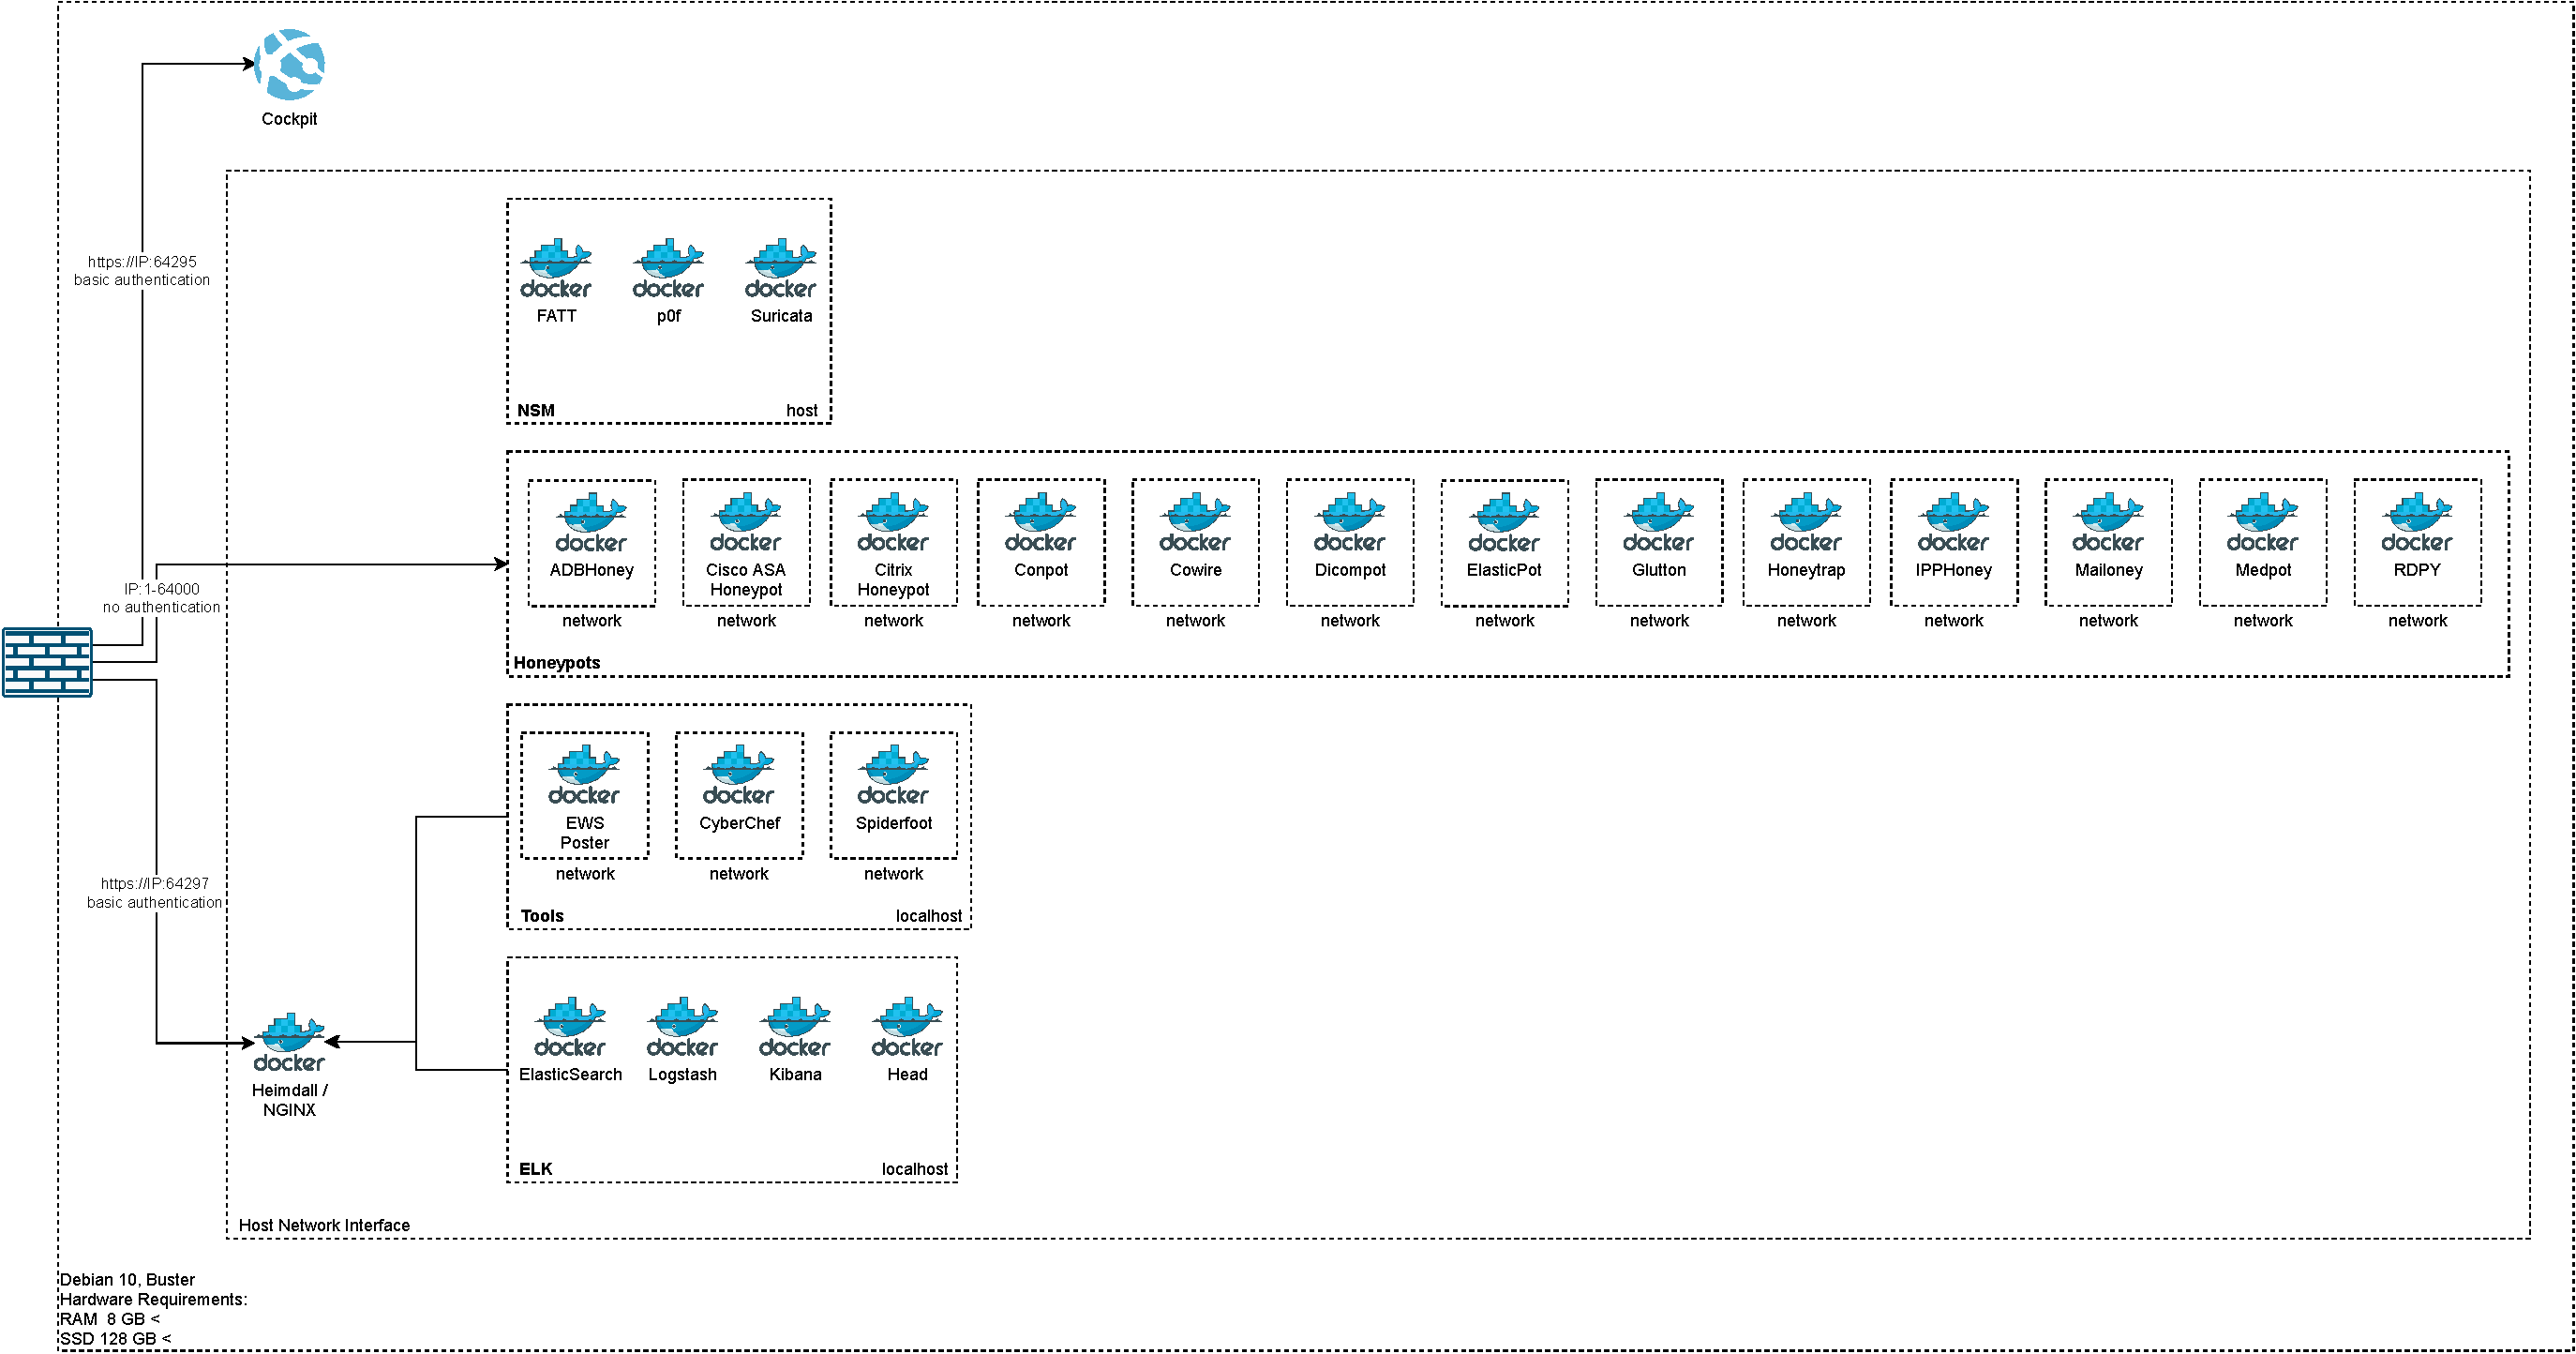
\includegraphics[width=\textwidth]{figures/tpot-architecture.pdf}
    \caption[T-Pot architecture]{T-Pot architecture derived from \cite{tpot2021}. Honeypots are encapsulated in their own network. NSM runs on the host network, and thus, receives every packet. ELK and tools run on localhost, and are accessible through NGINX.}
    \label{fig:overview-tpot}
\end{sidewaysfigure}

\subsubsection{Honeypots}

T-Pot consists of 20 honeypots. Albeit the sheer quantity of it, we will give a short explanation.
In addition, \autoref{tab:overview-honeypots} gives a quick overview of all available honeypots in conjunction with
\begin{enumerate*}[label=(\roman*)]
    \item the port they are running on,
    \item their interaction level, and
    \item a short description
\end{enumerate*}.

\textbf{ADBHoney} \cite{adbhoney2021} is a low interaction \ac{adb} honeypot over TCP/IP.
The importance of it lies in the \ac{adb} protocol that is used to debug and push content to Android device.
However, unlike USB it does not support any kind of ample mechanisms of authentication and protection.
By exposing the \ac{adb} service over any port, an adversary could connect and exploit it.
ADBHoney is designed to catch malware that has been pushed onto devices.

\textbf{Cisco \ac{asa}} \cite{cymmetria2018} is a low interaction honeypot that detects CVE-2018-0101\cite{CVE-2018-0101}.
It is a vulnerability that could allow an unauthenticated remote attacker to cause a reload of the affected system and to remotely execute code.
This can be achieved by flooding a webvpn-configured interface with crafted XML packets.
Consequently, the attacker obtain full control by executing arbitrary code.

\textbf{Citrix \ac{adc} honeypot} \cite{citrixhoneypot2020} detects and logs CVE-2019-19781\cite{CVE-2019-19781} scans and exploitation attempts.
This vulnerability allows adversaries to perform directory traversal attacks.
Files are accessible by path strings to denote the file or directory.
In addition, some file systems include special character to easily traverse the hierarchy.
Attackers take advantage of it by combining special characters in order to get access to restricted areas. \cite{flanders2019}

\textbf{Conpot} \cite{conpot2021} is a low interaction industrial honeypot for \ac{ics}, and \ac{scada}.
It provides a variety of different common industrial control protocols.
An adversary should be tricked by the complex infrastructure, and lure him into attacks.
In addition, a custom human machine interface can be connected to increase the attack surface.
By randomly delaying the response time, Conpot tries to emulate a real machine handling a certain amount of load.

\textbf{Cowrie} \cite{cowrie2021} is a medium to high interaction SSH and Telnet honeypot.
It offers to log brute-force attacks and shell interactions with attackers.
In medium interaction mode cowrie emulates a UNIX shell in Python, whereas in high interaction mode it proxies all commands to another system.

\textbf{DDoSPot} \cite{ddosspot2021} is a low interaction honeypot to log and detect UDP-based \ac{ddos} attacks.
It is used as a platform to support various plugins for different honeypot services, and servers.
Currently, it supports \acs{dns}, \acs{ntp}, \acs{ssdp}, \acs{chargen}, and random/mock UDP server.

\textbf{Dicompot} \cite{dicompot2021} is a low interaction honeypot for the \ac{dicom} protocol.
As other honeypots before, it mocks a \ac{dicom} server in Go to collect logs and detect attacks.

\textbf{Dionaea} \cite{dionaea2021} is a medium interaction honeypot that tries to capture malware copies by exposing services.
It supports a vast variety of protocols such as FTP, SMB, and HTTP.
Several modules can be integrated to work with Dionaea such as VirusTotal for further malware results.

\textbf{Elasticpot} \cite{elasticpot2021} is a low interaction honeypot for Elasticsearch, a search engine based on the Lucene library.

\textbf{Glutton} \cite{glutton2021} is a generic low interaction honeypot that works as a MitM for SSH and TCP.
However, lacking documentation does not provide a deeper inside of this honeypot.

\textbf{Heralding} \cite{heralding2021} is a credential catching honeypot for protocols like FTP, Telnet, SSH, HTTP, or IMAP.

\textbf{HoneyPy} \cite{honeysap2021} is a low to medium interaction honeypot that supports several protocols such as UDP, or TCP.
New protocols can be added by writing a custom plugin for it.
HoneyPy should give the freedom of easily deploying and extending honeypots.

\textbf{HoneySAP} \cite{honeysap2021} is a low interaction honeypot tailored for SAP services.

\textbf{Honeytrap} \cite{honeytrap2021} is a low interaction honeypot network security tool.
As stated by \citet*{honeytrap2021}, Honeytrap is vulnerable to buffer overflow attacks.

\textbf{IPPHoney} \cite{ipphoney2021} is a low interaction \ac{ipp} honeypot.

\textbf{Mailoney} \cite{mailoney2021} is a low interaction SMTP honeypot written in Python.

\textbf{MEDpot} \cite{medpot2021} is a low interaction honeypot focused on \ac{fhir}.
It is a standard description data format to transfer and exchange medical health records.

\textbf{RDPY} \cite{rdpy2021} is a low interaction honeypot of the Microsoft \ac{rdp} written in Python.
It features client and server side, and it based on the event driven network engine Twisted.
It supports authentication over SSL and NLA.

\textbf{SNARE and TANNER} \cite{snare2021, tanner2021} is a honeypot project.
SNARE is an abbreviation for Super Next generation Advanced Reactive honEypot.
It is a successor of Glastopf, a web application sensor.
In addition, it supports the feature of converting existing webpages into attack surfaces.
TANNER \cite{tanner2021} can be seen as SNARES's brain.
Whenever a request has been sent to SNARE, TANNER decides how the response should like.

\subsubsection{Tools}

T-Pot integrates tools to screen network traffic.

\textbf{FATT} \cite{fatt2021} is used to extract metadata and fingerprints such as JA3 \cite{ja32021} and HASSH \cite{hassh2021} from captured packets.
JA3 is a method for \enquote{creating SSL/TLS client fingerprints} whereas HASSH is a \enquote{network fingerprinting standard which can be used to identify specific client and server SSH implementations}.
In addition, it features live network traffic.
As noted by the author, FATT is based on a python wrapper for tshark, namely pyshark, and thus having performance downturns.
T-Pot applies FATT on every request made on the host network.

\textbf{Spiderfoot} \cite{spiderfoot2021} is an open source intelligence automation tool that helps to screen targets to get information about what is exposed over the Internet.
It can target different entities such as IP address, domain, hostname or network subnet.
In addition, it features more than 200 modules that can be integrated as an extension.
T-Pot uses it to scan defensively and thus not include any other module.

\textbf{Suricata} \cite{suricata2021} is \enquote{a high performance \ac{ids}, \ac{ips} and \ac{nsm} engine}.
T-Pot lets Suricata analyze and assess any request made on the host network.

\textbf{P0f} \cite{p0f2021} is a fingerprinting tool that uses passive traffic fingerprinting mechanisms to check TCP/IP communications.
T-Pot lets p0f passively check any request made on the host network.

\textbf{Endlessh} \cite{endlessh2021} is an SSH server that sends an endless, random SSH banner.
The key idea is to lock up SSH clients that try to connect to the SSH server.
It lowers the transaction speed by intentionally inserting delays.
Due to connection establishing before cryptographic exchange, this module does not require any cryptographic libraries.

\textbf{HellPot} \cite{hellpot2021} is an \enquote{endless honeypot}.
Connecting to this honeypot results in a memory overflow.
Its key idea is to send an endless stream of data to the attacker until its memory, or storage runs out.

\begin{sidewaystable}
    \centering
    \caption[Overview honeypots of T-Pot]{Overview of all available honeypots and tools of T-Pot with interaction level, port, and a short description. Ports are marked with either TCP or UDP, if a port misses any definition, both TCP and UDP are allowed.}
    \begin{tabularx}{\linewidth}{l|XlX}
        \toprule
        \textsc{Honeypots}                        & \multicolumn{3}{c}{}                                                                                                                                                                                                            \\
                                                  & \textbf{Port}                                                                                               & \textbf{Interaction-level} & \textbf{Description}                                                                 \\
        \hline
        ADBHoney \cite{adbhoney2021}              & 5555/TCP                                                                                                    & low                        & \ac{adb} protocol honeypot                                                           \\
        Cisco ASA \cite{cymmetria2018}            & 5000/UDP, 8443/TCP                                                                                          & low                        & honeypot for CVE-2018-0101\cite{CVE-2018-0101} detection                             \\
        Citrix honeypot \cite{citrixhoneypot2020} & 443/TCP                                                                                                     & low                        & detects and logs CVE-2019-19781\cite{CVE-2019-19781} scans and exploitation attempts \\
        Conpot \cite{conpot2021}                  & 80, 102, 161, 502, 623, 1025, 2404, \newline 10001, 44818, 47808, 50100                                     & low                        & industrial honeypot for \ac{ics}, and \ac{scada}                                     \\
        Cowrie \cite{cowrie2021}                  & 2222, 23                                                                                                    & high                       & SSH and Telnet honeypot                                                              \\
        DDoSPot \cite{ddosspot2021}               & 1112/TCP                                                                                                    & low                        & log and detect UDP-based \ac{ddos} attacks                                           \\
        Dicompot \cite{dicompot2021}              & 1112/TCP                                                                                                    & medium                     & honeypot for the \ac{dicom} protocol                                                 \\
        Dionaea \cite{dionaea2021}                & 21, 42, 69/UDP, 8081, 135, 443, 445, \newline 1433, 1723, 1883, 1900/UDP, \newline 3306, 5060/UDP, 5061/UDP & low                        & capture malware copies                                                               \\
        Elasticpot \cite{elasticpot2021}          & 9200                                                                                                        & low                        & honeypot for Elasticsearch                                                           \\
        Glutton \cite{glutton2021}                & NFQ                                                                                                         & medium                     & MitM proxy for SSH and TCP                                                           \\
        Heralding \cite{heralding2021}            & 21, 22, 23, 25, 80, 110, 143, 443, \newline 993, 995, 1080, 5432, 5900                                      & low                        & credential catching honeypot                                                         \\
        HoneyPy \cite{honeysap2021}               & 7, 8, 2048, 2323, 2324, 4096, 9200                                                                          & low                        & extendable honeypot                                                                  \\
        HoneySAP \cite{honeysap2021}              & 3299/TCP                                                                                                    & low                        & honeypot for SAP services                                                            \\
        Honeytrap \cite{honeytrap2021}            & NFQ                                                                                                         & medium                     & captures attacks via unknown protocols                                               \\
        IPPHoney \cite{ipphoney2021}              & 631                                                                                                         & low                        & \ac{ipp} honeypot                                                                    \\
        Mailoney \cite{mailoney2021}              & 25                                                                                                          & low                        & SMTP honeypot                                                                        \\
        MEDpot \cite{medpot2021}                  & 2575                                                                                                        & low                        & \ac{fhir} honeypot                                                                   \\
        RDPY \cite{rdpy2021}                      & 3389                                                                                                        & low                        & Microsoft \ac{rdp} honeypot                                                          \\
        SNARE/TANNER \cite{snare2021}             & 80                                                                                                          & low                        & web application honeypot                                                             \\
        \bottomrule
    \end{tabularx}
    \label{tab:overview-honeypots}
\end{sidewaystable}

\section{Results}% TODO: Fix data timestamp Sep 21 00:00 to Oct 16th 00:00, Recheck results
\label{sec:honeypots-heicloud}

Our T-Pot has been deployed for 3 weeks (from 21st of September to 16th of October) and collected in total \numprint{825,539} attacks.
Overall, RDPY ($47.94\%$), Honeytrap ($32.27\%$), and Cowrie ($12.60\%$) received most of the attacks with a total amount of \numprint{540,398} attacks.
\autoref{fig:overview-attacks} shows the distribution of honeypot attacks.
The total numbers are based on \autoref{tab:overview-honeypots-attacks}.

\begin{figure}[ht]
    \centering
    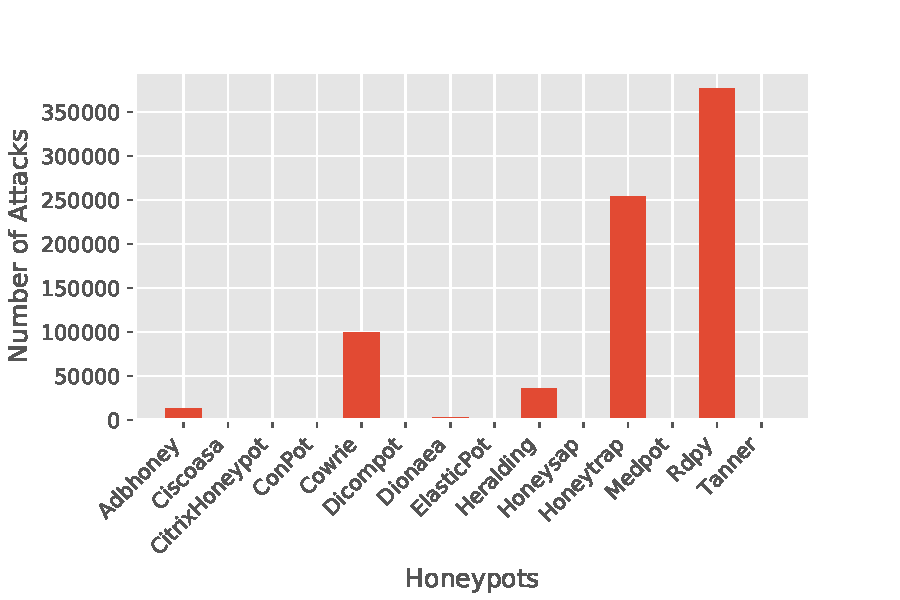
\includegraphics[width=\textwidth]{figures/tpot-overview-attacks.pdf}
    \caption[Distribution of honeypot attacks]{Distribution of honeypot attacks}
    \label{fig:overview-attacks}
\end{figure}

Noticeable is the large disparity of the previously mentioned attacks on \ac{aws}, \ac{gcp}, and Azure.
Especially for honeypots like Dionaea, it is shallow why so little attacks have been performed.
Therefore, we assume that packets run through a static filter.
Heidelberg itself has a centralized packet filtering which indicates our assumption that certain ports or protocols are excluded.
To prove that, a \textsc{nmap} TCP SYN scan (\verb|nmap -sS -A 129.206.5.74|) has been executed. % TODO: Write about uni firewall
Our result clearly shows that port 20, reserved for FTP, is filtered, although the access security explicitly allows it.
Based on this, most of the attacks on Dionaea are made throughout FTP, and thus, explains the total number of attacks.
Moreover, $96\%$ of IP addresses connected to Dionaea are known attackers, and $70\%$ were acquired on port 81, unofficially known for Tor routing.
Neither any malware nor suspicious payload could be identified.
Even with an \ac{acl} running in the background, heiCLOUD received more attacks than ever.
We assume that the real number might be even higher without packet filtering for FTP port 20.
However, due to security concerns a temporarily exclude of this rule has been rejected.

\begin{figure}[ht]
    \centering
    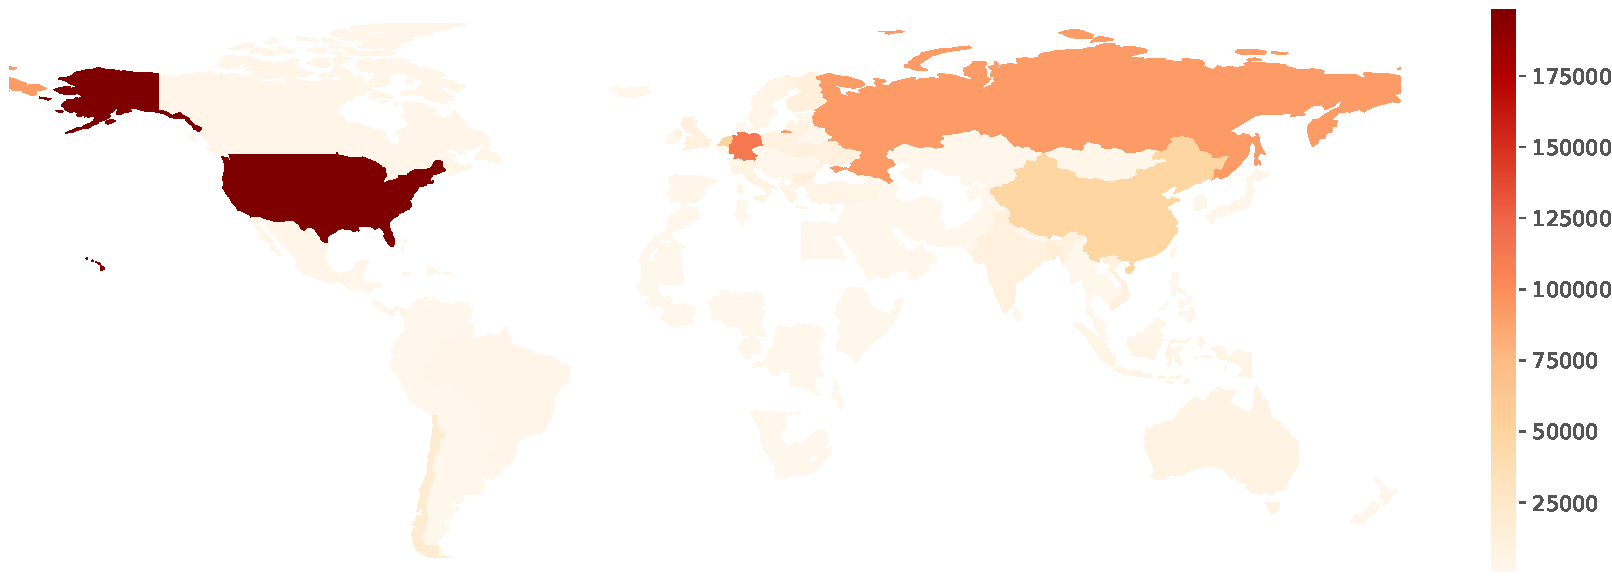
\includegraphics[width=\textwidth]{figures/tpot-overview-map.pdf}
    \caption[Attack distribution of T-Pot]{Attack distribution of T-Pot. USA, Russia, China, and Germany are the most attacking countries. Timestamp; 21st of September to 16th of October.}
    \label{fig:attack-distribution}
\end{figure}

Logstash uses GeoLite2 to resolve the source IP address with information such as location, ASN, continent code, country name, and AS organization.
\autoref{fig:attack-distribution} indicates the geographical location of connections acquired to any honeypot.
Most attacks are originated from the United States, Germany, Russia, and China.
Large security scans of DFN or \ac{belwue} pushes Germany on second place, therefore, Germany can be considered negligible.
On the contrary, the geographical location of an IP address merely indicates the true origin.
Due to technologies like VPN or Tor, the last known node of an IP address could be spoofed, and thus as stated by \citet{Kelly2021}, would remain insufficient to use.
Hence, we do not strongly rely on the geographical information.

\begin{figure}[ht]
    \centering
    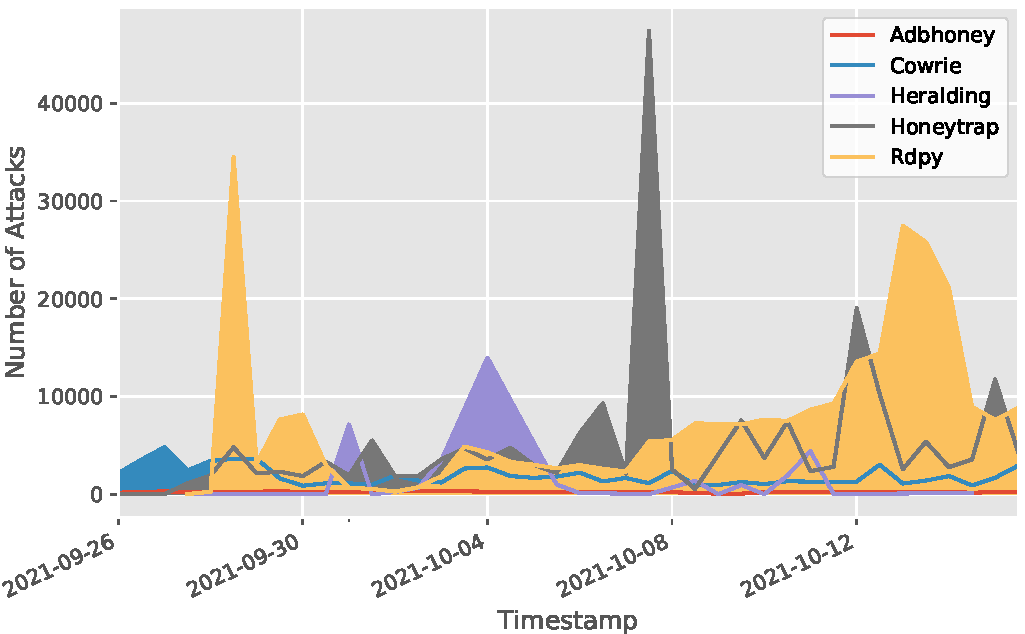
\includegraphics[width=\textwidth]{figures/tpot-attacks-histogram.pdf}
    \caption[Attack histogram of T-Pot]{Attack histogram of T-Pot. Only the five most attacked honeypots are considered. Timestamp; 21st of September to 16th of October.}
    \label{tpot-overview-histogram}
\end{figure}

Attacks are not equally distributed among all honeypots, and thus, different protocols and application receive more attention than others.
\autoref{tpot-overview-histogram} shows the timeline of attacks that are executed on our instance separated by honeypots.
RDPY, Honeytrap, and Cowrie are clearly the most attacked honeypots.
The high peak of Honeytrap in the middle indicates a full \textsc{nmap} scan from Germany that has been done to get an inside of the packet filtering at the Heidelberg University.
We clearly identify a bias towards remote desktop protocol attacks, shell-code exploitation, and commands to retrieve information about CPU, scheduled tasks (\verb|cat /proc/cpuinfo|, or \verb|crontab|), or privilege escalation.

\begin{figure}[ht]
    \centering
    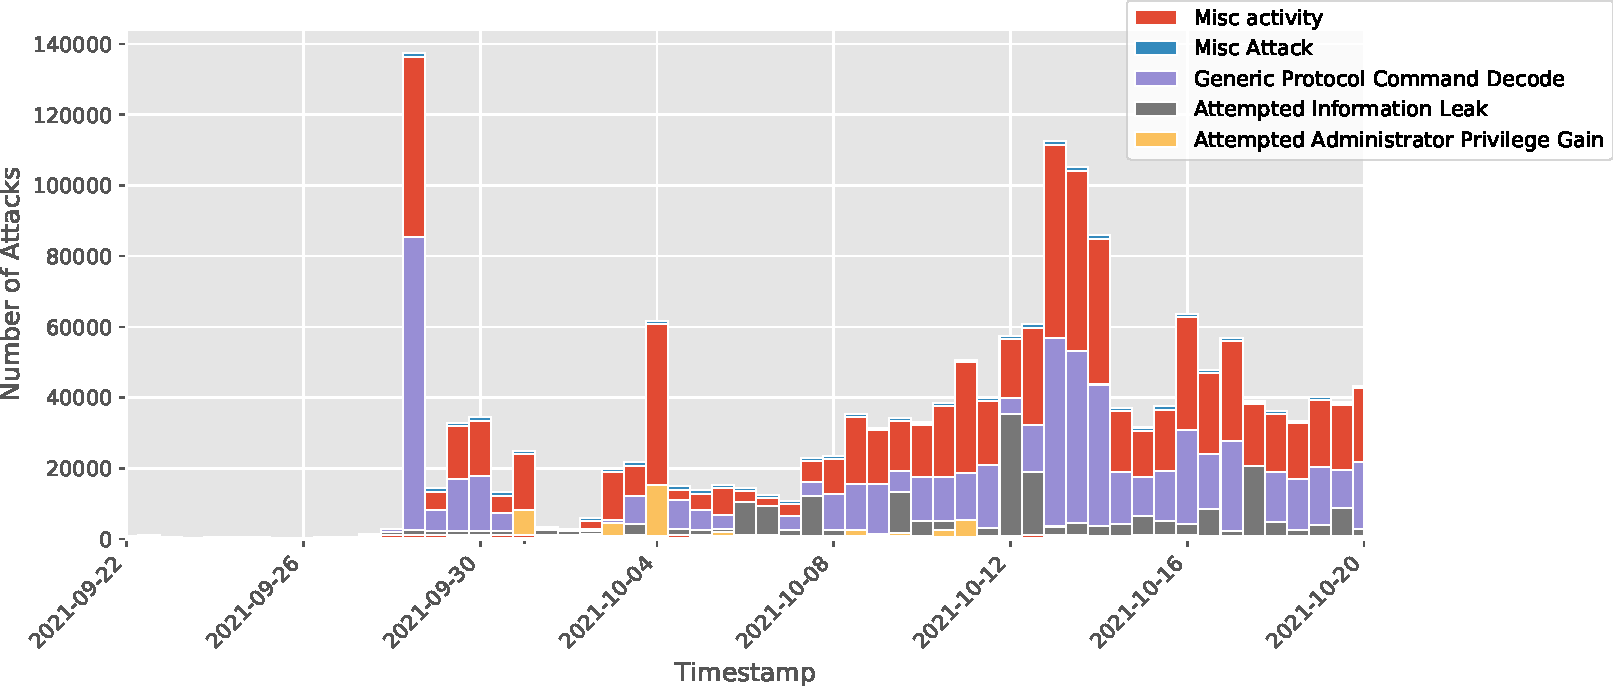
\includegraphics[width=\textwidth]{figures/tpot-suricata-alerts.pdf}
    \caption[Suricata results of T-Pot]{Suricata results of T-Pot. Displays the five most listed alert categories. Timestamp; 21st of September to 16th of October.}
    \label{fig:suricata-results}
\end{figure}

Suricata registered several alerts and CVE's.
The vast majority of alerts are RDP related policies, VNC authentication failures, and \textsc{nmap} scans.
Most used vulnerabilities are
\begin{enumerate*}[label=(\roman*)]
    \item CVE-2001-0540\cite{CVE-2001-0540} which is a memory leak in Terminal servers in Windows NT and Windows 2000 causing a denial of service (memory exhaustion) by malformed RDP requests,
    \item CVE-2006-2369\cite{CVE-2006-2369} which is a RealVNC vulnerability allowing hackers to bypass authentication, and
    \item CVE-2012-0152\cite{CVE-2012-0152} which enables attackers for RDP in Microsoft Windows Server 2008 R2 and R2 SP1 and Windows 7 Gold and SP1 to cause a denial of service by sending a series of crafted packets
\end{enumerate*}.
As derived from \autoref{fig:suricata-results}, our T-Pot have not received many attacks in the first week.
Starting from 28th of October the numbers of alert are skyrocketing.
This would indicate that bots crawl IP address ranges to find new machines and probe them.
Interestingly, zero-day exploits like the Apache vulnerability \cite{CVE-2021-42013} that came with version $2.49.0$ got registered in CVE on the 6th of October, and immediately recognized by Suricata on the 15th of October.
Attackers could perform a remote code execution using path traversal attacks when the CGI scripts of Apache are enabled.
We could trace back similar attacks like \verb|/cgi-bin/.\%2e/\%2e\%2e/bin/sh| until the 7th of October, leaving an even smaller time frame to adapt to new exposures.
This shows how fast bots adapt to new vulnerabilities in order to compromise more systems.

\begin{figure}[ht]
    \centering
    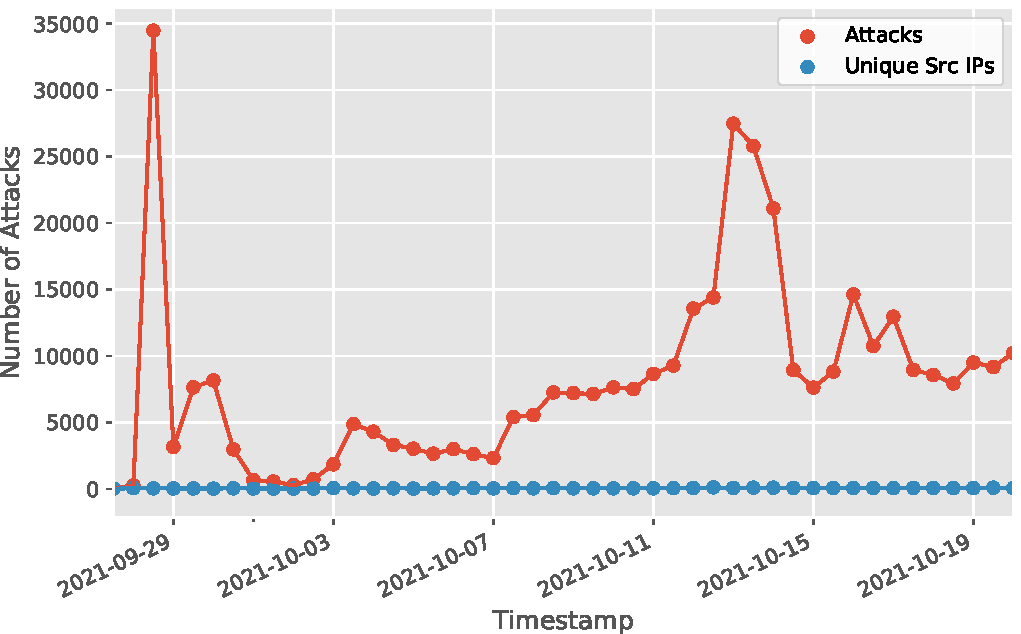
\includegraphics[width=\textwidth]{figures/tpot-rdpy-port.pdf}
    \caption[RDPY results of T-Pot]{RDPY attacks separated in attacks and unique src IPs. Timestamp; 21st of September to 16th of October.}
    \label{fig:rdpy-results}
\end{figure}

The results from RDPY in \autoref{fig:rdpy-results} backups our assumption.
It shows that only a small margin represents unique src IPs.
The rest of the attacks result in either bad reputation, bot, crawler, or known attacker.
\autoref{fig:suricata-results} shows the distribution of alert categories that Suricata identified.
Respectively, misc activities sum up to roughly $1.5$ million entries, \ac{rdp} related alerts account two-third of it.
Several RDP attacks from 2021 back to 2001 had been executed on our T-Pot.
Respectively, CVE-2012-0152 and CVE-2001-0540 coincide with the ones \citet{Kelly2021} claim.
We assume the skyrocketing number of attacks roots back to the Corona pandemic due to an increase of the remote desktop protocol.
Furthermore, lack of updates and outdated servers using \ac{rdp} remain an ease target for automatic attacks that scan the web and try to find new exposures.

\begin{figure}[ht]
    \centering
    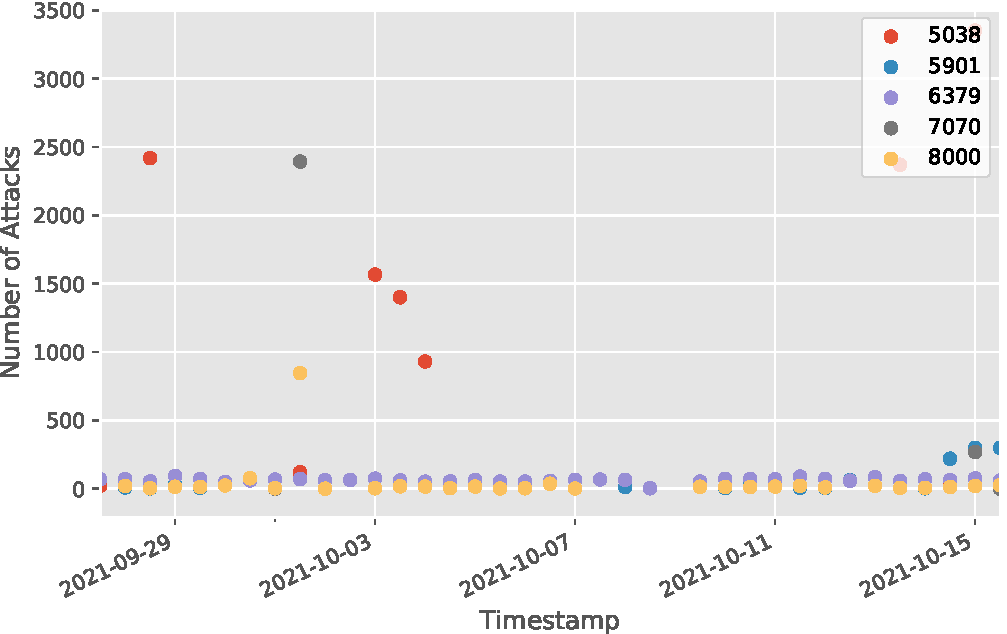
\includegraphics[width=\textwidth]{figures/tpot-honeytrap-port.pdf}
    \caption[Honeytrap results of T-Pot]{Honeytrap results of T-Pot. Timestamp; 21st of September to 16th of October.}
    \label{fig:honeytrap-results}
\end{figure}

For NFQ related attacks, Honeytrap could identify three major services that are not provided by default.
Honeytrap functions as a honeypot to provide a service on ports which are not specified by default.
NFQ intercepts incoming TCP connections during the TCP handshake and let Honeytrap providing a service for it.
Most of these interceptions are made on
\begin{enumerate*}[label=(\roman*)]
    \item port 5038 which is merely used by a machine learning database called MLDB,
    \item port 5905 which is merely used by an Intel Online Connect Access on Windows machines, and
    \item port 7070 which is merely used by Apple's QuickTime streaming server (RTSP)
\end{enumerate*}.
On nearly all ports attacks focused on RDP connection attempts (\verb|Cookie: mstshash=Administr|).
However, $94\%$ of all connected IP addresses are resolved as known attackers.

\begin{figure}[ht]
    \centering
    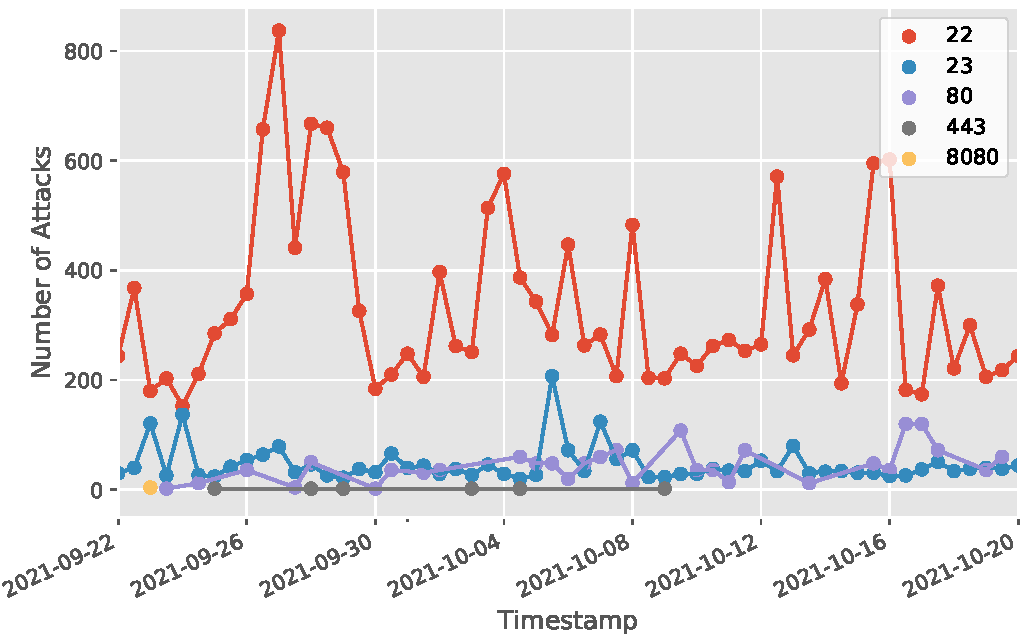
\includegraphics[width=\textwidth]{figures/tpot-cowrie-port.pdf}
    \caption[Cowrie results of T-Pot]{Cowrie results of T-Pot. Timestamp; 21st of September to 16th of October.}
    \label{fig:cowrie-results}
\end{figure}

Third most compromised honeypot is Cowrie with a strong bias towards SSH, and FTP.
\autoref{fig:cowrie-results} shows all attacks executed on Cowrie separated by their port.
Respectively, SSH port $22$ is the most considered port, resulting in a high use for privilege escalation.
Besides default credentials login attempts (\verb|username: root|, \verb|password: root|, see \autoref{fig:cowrie-credentials} for top 10 credentials), adversaries used various commands to retrieve any information about the host system (\verb|nproc;uname -a|, \verb|cat /proc/cpuinfo|).
We could identify a unique information gathering attack that has been widely used on our T-Pot.
\autoref{lst:code-exploitation} shows all shell commands that are executed.
Attackers try to gain knowledge about the running process on the system (\verb|/bin/busybox|).
Interestingly, crypto mining attacks are getting more attractive to criminals.
As an example, XMRig has been the most downloaded malware for cryptocurrency mining.
Some adversaries even executed complex tailored shell commands to exploit the host machine as a crypto miner (\autoref{lst:crypto-exploitation}).
With respect to the current time it is not surprising that such attacks gain attraction.
Attackers could exploit machines for crypto mining in order to earn more money.
This looks more appealing than acquiring mining machines and hijacking electricity from surrounding apartments (Quelle!).

\begin{figure}
    \lstinputlisting[language=bash, caption={Cowrie attack to gather various information about the system}, label={lst:code-exploitation}]{listings/exploit-cpu.sh.txt}
\end{figure}

\begin{figure}
    \lstinputlisting[language=bash, caption={Cowrie attack to exploit the host machine as a crypt miner}, label={lst:crypto-exploitation}]{listings/exploit-crypt.sh.txt}
\end{figure}

\begin{figure*}
    \centering

    \begin{subfigure}[b]{0.49\textwidth}
        \centering
        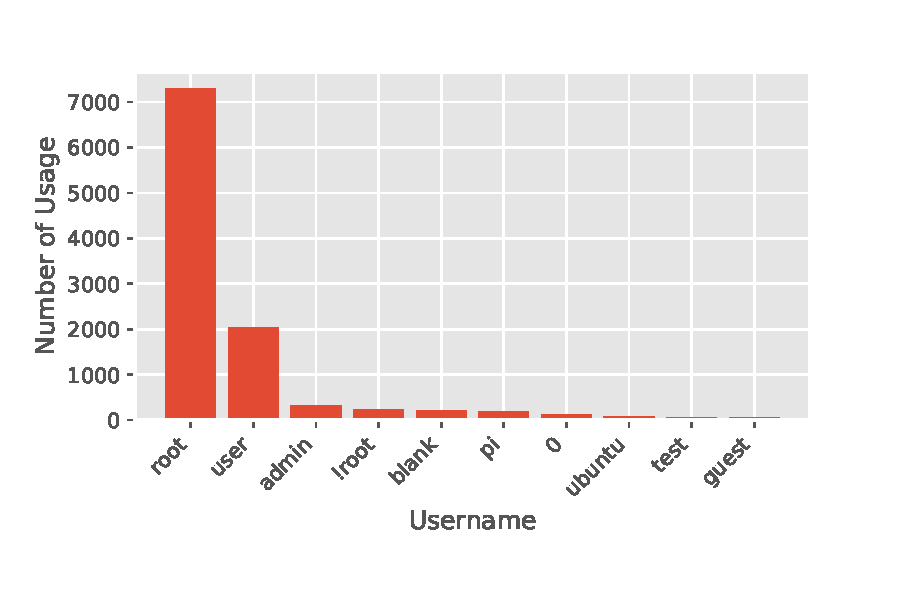
\includegraphics[width=\textwidth]{figures/tpot-cowrie-username.pdf}
        \caption{Cowrie username credentials}
        \label{fig:tpot-cowrie-username}
    \end{subfigure}
    \hfill
    \begin{subfigure}[b]{0.49\textwidth}
        \centering
        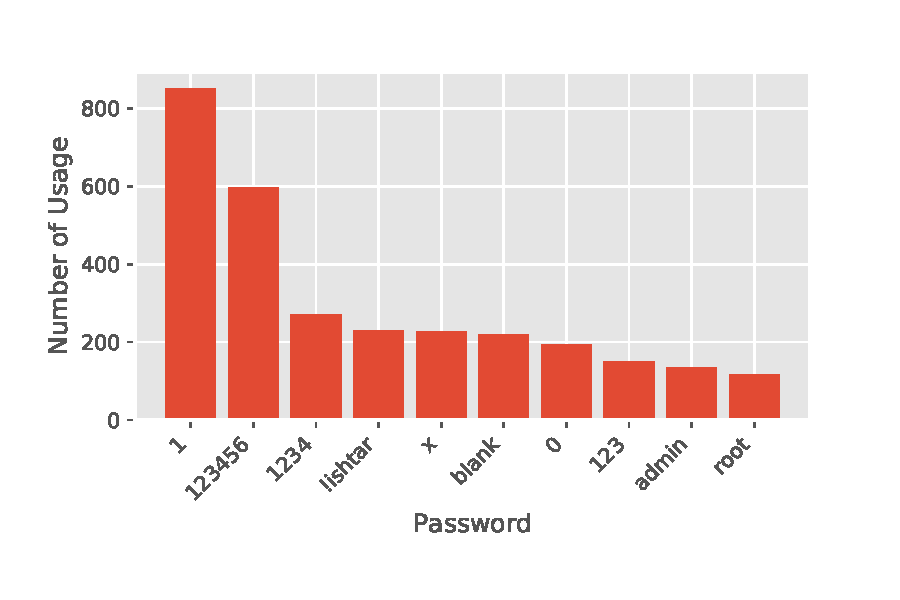
\includegraphics[width=\textwidth]{figures/tpot-cowrie-password.pdf}
        \caption{Cowrie password credentials}
        \label{fig:tpot-cowrie-password}
    \end{subfigure}
    \caption[Cowrie top 10 credentials on T-Pot]{Cowrie top 10 credentials used on T-Pot. Timestamp 22nd of September to 18th of October}
    \label{fig:cowrie-credentials}
\end{figure*}

P0f identified different Windows versions and Linux distributions in conjunction with various SSH clients that are used to compromise our T-Pot.
Like \citet{Kelly2021}, Windows 7 or 8 and Windows NT Kernel are the most used \ac{os} with $81\%$.
Unfortunately, disguising OS fingerprinting activities account $84\%$.
Lastly, we cleaned up our results and excluded all IPs from DFN and \acs{belwue} from our results.
Both do frequent scans and check if any vulnerability exists.
This distorts our findings, and thus, we filtered them based on their subnet addresses.
However, the results show no big changes.
The total number of attacks were merely influenced by it.
This indicates that our own scans do not greatly interfere with our findings.
Due to completeness, we leave our results as they are and do not show the filtered data.

% Conclusion
Overall, heiCLOUD has nearly doubled the size of attacks.
On average, heiCLOUD has received $195.31\%$ more than Azure, \ac{gcp}, and \ac{aws}.
Attacks on Cowrie, RDPY, and Honeytrap are the most compromised honeypots.
In contrast to \citet{Kelly2021}, Dionaea and Glutton used to be the most considered honeypots for adversaries.
We assume that attacks by bots have increased significantly since last year when \citet{Kelly2021} did their research.
Respectively, one question we are not able to answer is if other cloud providers filter their network traffic.
It would explain the major difference between Heidelberg University and the big tech companies.
The cause for such an increase remains doubtful.
One explanation could root back to the Corona pandemic and the skyrocketing increase in home office activities.
Related to that is a higher usage in screen sharing software.
Considering the BSI\footnote{The Federal Office for Information Security is responsible for managing communication security for the German government. Each year they publish a report for recent cybersecurity threats.} report for cybersecurity 2021 \cite{bsi2021}, they revealed an increase of attack surfaces during the pandemic.
Respectively, the IT infrastructure could not keep up with this fast change and widen the attack surface of the company.
Their conclusion overlays our assumption that attackers took advantage and increase their activities.
This phenomenon shows that nearly all attacks originate from bots which scan through IP address ranges.
In total, $73\%$ of all IP address are unresolved, known attacker reputation represents the largest part of resolved IP addresses with $23\%$.
Fortunately, such reputations could technically be filtered by an organization's firewall and would lower the chance of an exploit.
Interestingly, after 3 weeks the number of attacks originated from China decreased to almost zero percent.
This might be an indication that our honeypot has been exposed, and further attacks represent a risk of revealing their compromises.
However, this assumption cannot be confirmed due to the lax geographical reliability of IP addresses.

Our results lay emphasis on the importance of honeypots.
It shows that recent bot activities can be traced to find the newest trends of attacks.

\begin{sidewaystable}
    \centering
    \caption[Overview of attacks on cloud providers]{Overview of attacks on heiCLOUD, AWS, GC and Azure. Only the top 10 most attacked honeypots are considered. \enquote{-} entails that a honeypot is not part of the top 10.}
    \begin{tabularx}{\linewidth}{l|XXc|XX|XX|XX}
        \toprule
        \textsc{Honeypots} & \multicolumn{3}{c}{BASIS}              & \multicolumn{6}{c}{\textsc{comparison}}                                                                                                                                                             \\
                           & \multicolumn{3}{c|}{\textsc{heiCLOUD}} & \multicolumn{2}{c|}{\textsc{AWS}}       & \multicolumn{2}{c|}{\textsc{GC}} & \multicolumn{2}{c}{\textsc{Azure}}                                                                                     \\
                           & \textbf{Number}                        & \textbf{Pct.}                           &                                  & \textbf{Number}                    & \textbf{Pct.} & \textbf{Number} & \textbf{Pct.} & \textbf{Number} & \textbf{Pct.} \\
        \hline
        ADBHoney           & $13292$                                & $1.65\%$                                & $\color{green}{\uparrow}$        & 413                                & $0.13\%$      & 2497            & $0.43\%$      & 442             & $0.13\%$      \\
        Cisco ASA          & $944$                                  & $0.11\%$                                & $\color{green}{\uparrow}$        & 260                                & $0.08\%$      & 750             & $0.13\%$      & 134             & $0.04\%$      \\
        Citrix honeypot    & $1471$                                 & $0.18\%$                                &                                  & -                                  & -             & -               & -             & -               & -             \\
        Conpot             & $1003$                                 & $0.10\%$                                &                                  & -                                  & -             & -               & -             & -               & -             \\
        Cowrie             & $990069$                               & $11.97\%$                               & $\color{red}{\downarrow}$                                 & 4503                               & $1.46\%$      & 297818          & $51.25\%$     & 9012            & $2.64\%$      \\
        DDoSPot            & $0$                                    & $0\%$                                   &                                  & -                                  & -             & -               & -             & -               & -             \\
        Dicompot           & $25$                                   & $0\%$                                   &                                  & -                                  & -             & -               & -             & -               & -             \\
        Dionaea            & $3110$                                 & $0.40\%$                                & $\color{red}{\downarrow}$                                 & 288075                             & $93.49\%$     & 162570          & $27.98\%$     & 308102          & $90.42\%$     \\
        Elasticpot         & $512$                                  & $0.06\%$                                &                                  & -                                  & -             & -               & -             & -               & -             \\
        Glutton            & $0$                                    & $0\%$                                   & $\color{red}{\downarrow}$                                 & 11878                              & $3.85\%$      & 84375           & $15.52\%$     & 17256           & $5.06\%$      \\
        Heralding          & $35836$                                & $4.34\%$                                & $\color{green}{\uparrow}$                                 & 1885                               & $0.61\%$      & 12255           & $2.11\%$      & 3370            & $0.99\%$      \\
        HoneyPy            & $0$                                    & $0\%$                                   & $\color{red}{\downarrow}$                                 & 172                                & $0.06\%$      & 2149            & $0.37\%$      & 497             & $0.15\%$      \\
        HoneySAP           & $18$                                   & $0\%$                                   &                                  & -                                  & -             & -               & -             & -               & -             \\
        Honeytrap          & $253854$                               & $32.01\%$                               &                                  & -                                  & -             & -               & -             & -               & -             \\
        IPPHoney           & $0$                                    & $0\%$                                   &                                  & -                                  & -             & -               & -             & -               & -             \\
        Mailoney           & $0$                                    & $0\%$                                   & $\color{red}{\downarrow}$                                 & 720                                & $0.23\%$      & 9419            & $1.62\%$      & 146             & $0.04\%$      \\
        MEDpot             & $3$                                    & $0\%$                                   &                                  & -                                  & -             & -               & -             & -               & -             \\
        RDPY               & $377045$                               & $49.15\%$                               &  $\color{green}{\uparrow}$                                & 100                                & $0.03\%$      & 7916            & $1.36\%$      & 1463            & $0.43\%$      \\
        SNARE/TANNER       & $382$                                  & $0.02\%$                                & $\color{red}{\downarrow}$                                 & 138                                & $0.04\%$      & 1367            & $0.24\%$      & 313             & $0.09\%$      \\
        \hline
        \textsc{In total}  & $786564$                               & $100\%$                                 &                                  & 308144                             & $100\%$       & 581116          & $100\%$       & 340735          & $100\%$       \\
        \bottomrule
    \end{tabularx}
    \label{tab:overview-honeypots-attacks}
\end{sidewaystable}

\section{Discussion}

One downside of T-Pot is the static hostname representation of Cowrie.
It always returns \verb|#1 SMP Debian 3.2.68-1+deb7u1| (\verb|uname -a|) as hostname information, leaving a tiny footprint when bots crawl through the web.
A random choice of hostname information could harden Cowrie from being exposed.
Next, if attackers would scan open ports on T-Pot, it might be suspicious when many ports with services are widely open.
From a technical perspective, bots could check this state if it is uncommon, and thus, exclude T-Pot from being probed.
However, T-Pot includes good preventions like random hostname and scheduled tasks.
Another major drawback is the latest endeavor to fingerprint honeypots.
As recently investigated by \citet{vetterl2020}, fingerprinting honeypots is becoming easier due to a fatal flaw in the underlying protocol implementation.
\citet{vetterl2020} states that attackers always try to prevent their methods, exploits and tools from being divulged.
Therefore, detecting honeypots before attack them is a strong motivation for black hats.
In \autoref{chap:fingerprinting} we will present a way to avoid fingerprinting of Cowrie.
